\documentclass{article}
\usepackage[margin=0.75in]{geometry}
\usepackage{graphicx}

\title{Baryon Imbalance}
\author{Andr\'{e}s N. Salcedo}
  
\begin{document}

\maketitle

The Big Bang should have created equal amounts of matter and antimatter and yet barely any antimatter is observed. Neither general relativity or the standard model offer explanations for this imbalance. This problem is referred to as the baryon asymmetry problem. One possible explanation is that matter and antimatter dominate different large scale regions of the universe. At astronomical distances matter and antimatter are indistinguishable but at the boundaries between these regions annihilation would occur offering an observational test of this theory. 

\begin{enumerate}

\item Estimate the number density of the IGM.

\item Estimate the particle collision rate in the IGM, as well as the matter-antimatter collision rate assuming equal amounts of each.

\item Assume that we are at the center of a spherical region of space dominated by matter. Write an expression for the gamma ray flux associated with matter-antimatter annihilations recieved as a function of distance to this boundary (assuming equal matter and antimatter).

\item If we observed a radiation background of energy $3 \times 10^5 \; \mathrm{keV}$ and of brightness $I = 10^{-4} \; \mathrm{cm^{-2}} \; \mathrm{s^{-1}} \; \mathrm{sr^{-1}}$ that we could be pretty sure is from annihilation at a matter-antimatter boundary what would this imply about the value of $\Omega_b$ and the scale of our matter dominated region (again assume equal matter and antimatter)?

\item Based on the data given write an expression relating $\Omega_b$, and the redshift of the hypothesized boundary. If we take $\Omega_b = 0.04$ what limiting distance to the hypothesized boundary does that require?

\end{enumerate}


\begin{figure}
\begin{center}
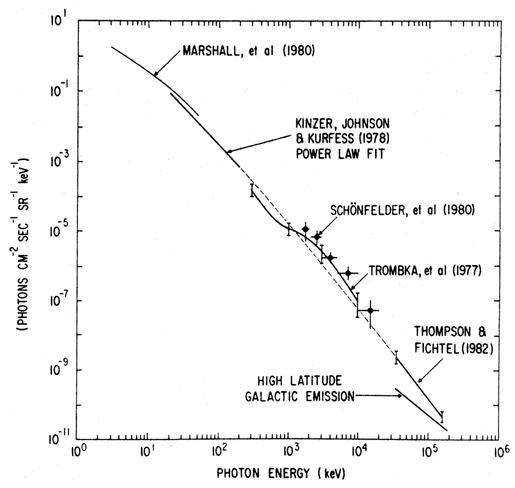
\includegraphics[width = 0.70\textwidth]{gamma_ray_background_spectrum.png}
\caption{Gamma-ray background surface brightness spectrum (From Trombka and Fichtel 1983).}
\end{center}
\end{figure}

\end{document}
